\section{Case Study}
\label{sec:case_study} 

% A aceitação de estudos empíricos em engenharia de software e suas contribuições para o aumento do conhecimento está crescendo continuamente \cite{runeson2009}. Para a validação da arquitetura proposta foi realizado um estudo de caso que consiste na avaliação do principal caso de uso do SISDOT, responsável pela geração de QDMs. O estudo de caso tem como objetivo responder às seguintes questões de pesquisa:

The acceptance of empirical studies in software engineering and its contributions to increasing knowledge is growing steadily \cite{runeson2009}. For the validation of the proposed architecture a case study was carried out, which consists of the evaluation of the main use case of SISDOT, responsible for the generation of QDMs. The case study aims to answer the following research questions:

\begin{itemize}

% \item \textbf{RQ.1}: O uso da DSL na execução de testes reduz o esforço do profissional de testes durante a implementação dos casos de testes?
\item \textbf{RQ.1}: Does the use of DSL in the execution of tests reduce the effort of the test professional during the implementation of the test cases?

% \item \textbf{RQ.2}: A solução de arquitetura adotada gera QDMs em um tempo considerado satisfatório pelo EB?
\item \textbf{RQ.2}: Does the adopted architecture solution generate QDMs at a time considered satisfactory by EB?

%\textcolor{red}{Acho que a frase precisa ser completada: A solução adotada gera QDMs no tempo adequado para uso em xxxx (tal coisa)}

%\item \textbf{RQ.3}: A transformação de chamadores em regras DRL gera uma quantidade de linhas de código satisfatória?
% \item \textbf{RQ.3}: Com a transformação de chamadores em regras DRL a solução proposta gera QDMs de acordo com o esperado/corretos?
\item \textbf{RQ.3}: With the transformation of callers into DRL rules does the proposed solution generate QDMs as expected/correct?

\end{itemize}

% A RQ.1 está relacionada à produtividade do testador e demonstra quanto código a menos o desenvolvedor deve implementar ao utilizar a DSL criada, em comparação com a declaração do mesmo chamador utilizando a linguagem Java. Apesar de não haver formalmente um requisito funcional especificando qual seria um tempo aceitável para a geração de um QDM, foi determinado que um tempo maior que 5 segundos, ao utilizar 1000 chamadores, é inaceitável. Assim, a RQ.2 serve para garantir que os QDMs sejam gerados em tempo satisfatório.

\textbf{RQ.1} is related to the productivity of the tester and demonstrates how much code the developer must implement when using the DSL created, compared to the caller's declaration using the Java language. Although there is no formal functional requirement specifying what would be an acceptable time for generating a QDM, it has been determined that a time greater than 5 seconds, when using 1000 callers, is unacceptable. Thus, \textbf{RQ.2} serves to ensure that the QDMs are generated in a satisfactory time.

% Com a RQ.3 pretende-se demonstrar que a solução gera as regras automaticamente, eliminando o trabalho que o desenvolvedor teria para implementar a solução em Java. Com poucas linhas de código, relacionadas à definição do template e sua execução, a solução gera um arquivo de regras com determinado número de linhas de código Drools. A resposta dessa questão está relacionada aos resultados dos testes manuais e automáticos.

With \textbf{RQ.3} it was intended to demonstrate that the solution automatically generates the rules, eliminating the work that the developer would have to implement the solution in Java. With a few lines of code related to the definition of the template and its execution, the solution generates a rule file with a number of Drools code lines. The answer to this question is related to the results of the manual and automatic tests.

\subsection{Data Collection}

% A coleta dos dados foi realizada utilizando as seguintes métricas: linhas de código (LOC) e tempo de execução. A escolha dessas duas métricas está relacionada ao tamanho do código, que pode indicar uma maior produtividade; e à satisfação do requisito funcional que determina o tempo máximo de execução para a geração de QDM. 

Data collection was performed using the following metrics: lines of code (LOC) and execution time. The choice of these two metrics is related to the size of the code, which may indicate higher productivity; and to the satisfaction of the functional requirement that determines the maximum execution time for the generation of QDM.

%A Tabela \ref{table:comparacao} apresenta a comparação dos resultados obtidos utilizando DSL e Java. 

\begin{table}[htb!]
\centering
\caption{Comparing the number of lines of code between DSL and Java}
\label{table:comparacao}
\begin{center}
\begin{tabular}{lll}
\hline
\textbf{Code} & \textbf{DSL} & \textbf{Java}     \\ \hline 
1        & 10  & 26   \\ \hline
2        & 10  & 25   \\ \hline
3        & 10  & 32   \\ \hline
4        & 11  & 52   \\ \hline
5        & 15  & 41   \\ \hline
6        & 9   & 16   \\ \hline
7        & 18  & 21   \\ \hline
8        & 12  & 25   \\ \hline
15       & 7   & 45   \\ \hline
58       & 7   & 58   \\ \hline
59       & 17  & 34   \\ \hline
\end{tabular}
\end{center}
\end{table}

% No cenário de testes considerado para o estudo de caso, o sistema SISDOT possuia  66 chamadores declarados em sua base de dados. Esses chamadores correspondem a chamadores reais utilizados pelo Exército Brasileiro (EB) para a realização de alguns testes na geração de QDMs. A conversão de cada chamador escrito na linguagem Java para o seu correspondente no formato da DSL foi realizada com o uso do Xtext. A Table \ref{table:comparacao} apresenta uma amostra dos dados coletados. A primeira coluna contém o código do chamador, a segunda coluna contém a quantidade de linhas de código para representar o chamador na DSL e a terceira coluna contém a quantidade de linhas para representar o mesmo chamador na linguagem Java.

In the test scenario considered for the case study, the SISDOT system had 66 callers declared in its database. These callers correspond to real callers used by the Brazilian Army (EB) to perform some tests in the generation of QDMs. The conversion of each caller written in the Java language to their correspondent in the DSL format was accomplished using Xtext. Table \ref{table:comparacao} presents a sample of the collected data. The first column contains the caller code, the second column contains the number of lines of code to represent the caller in the DSL, and the third column contains the number of lines to represent the same caller in the Java language.

% Para a coleta da métrica de tempo de execução foi utilizado um computador com processador Intel(R) Core(TM) i7-4790, com 16GB de memória RAM, com o sistema operacional Ubuntu 16.04.4 LTS, 64 bits, com kernel 4.15.0-24-generic. Foram usados 16 QCs, escolhidos de forma a representar os variados tipos de OM, naturezas e subnaturezas. Para cada QC foram gerados QDMs usando as seguintes quantidades de chamadores: 20, 40, 50, 60, 100, 200, 400, 700, 1000, 1500, 2000, 3000, 5000. Como só haviam 66 chamadores reais já declarados, os conjuntos com quantidade maior contém chamadores repetidos. A seleção dos chamadores foi realizada de maneira randômica, mas com o mesmo seed, para que os mesmos conjuntos fossem utilizados nas gerações dos QDMs de diferentes QCs. A Table \ref{table:tempo} apresenta uma amostra dos resultados obtidos com a execução. A primeira coluna contém o código do QC, e da segunda coluna em diante contém o tempo, em milisegundos, para a geração dos QDMs usando a quantidade de chamadores indicada no header da respectiva coluna.

For the collection of the runtime metrics, a computer with an Intel(R) Core{TM} i7-4790 processor, with 16GB of RAM, was used with the Ubuntu 16.04.4 LTS 64-bit operating system, with 4.15.0-24-generic kernel. We used 16 QCs, chosen to represent the various OM types, natures and subnatures. For each QC, QDMs were generated using the following quantities of callers: 20, 40, 50, 60, 100, 200, 400, 700, 1000, 1500, 2000, 3000, 5000. Since there were only 66 real callers already declared, with larger quantity contains repeated callers. The selection of callers was performed in random manner, but with the same seed, so that the same sets were used in the generation of QDMs different QCs. Table \ref{table:tempo} shows a sample of the results obtained with execution. The first column contains the QC code, and the second column contains on time in milliseconds for the generation of QDMs using the indicated amount of callers on the respective column header.

\begin{table}[htb!]
\centering
\caption{Time (ms) for generation of QDMs}
\label{table:tempo}
\begin{center}
\begin{tabular}{|l|l|l|l|l|l|l|}
\hline
\textbf{QC}      & \textbf{60}  & \textbf{100} & \textbf{400}  & \textbf{700}  & \textbf{1000} & \textbf{2000} \\ \hline

206410  & 184 & 275 & 944  & 1829 & 2279 & 4707 \\ \hline
231303  & 197 & 282 & 975  & 1731 & 2541 & 4987 \\ \hline
500311  & 201 & 291 & 948  & 1804 & 2289 & 4950 \\ \hline
618322  & 175 & 264 & 922  & 1640 & 2412 & 4990 \\ \hline
727310  & 173 & 302 & 937  & 1652 & 2466 & 4992 \\ \hline
1450311 & 182 & 269 & 890  & 1649 & 2527 & 4785 \\ \hline
2203310 & 197 & 263 & 909  & 1619 & 2344 & 4976 \\ \hline
5406194 & 176 & 253 & 884  & 1598 & 2393 & 4610 \\ \hline
7020003 & 212 & 241 & 922  & 1610 & 2361 & 4470 \\ \hline
9131000 & 171 & 252 & 888  & 1609 & 2345 & 4471 \\ \hline
\end{tabular}
\end{center}
\end{table}

\subsection{Data Analysis}

% Os dados coletados foram exportados no formato CSV para que pudessem ser analisados com maior facilidade com o uso de R \cite{crawley2013}. Na análise dos dados relativos à RQ.1, que compara a quantidade de linhas de código entre as representações dos chamadores em linguagem Java e na DSL, foram criadas colunas adicionais: diferença, que é a diferença no números de linhas de código entre Java e DSL; e percent\_menor, que indica o quanto o chamador DSL é menor que o mesmo chamador utilizando Java.

The collected data were exported in CSV format so that they could be analyzed more easily with the use of R \cite{crawley2013}. In the data analysis for \textbf{RQ.1}, which compares the number of lines of code between the representations of callers in Java language and in DSL, additional columns were created: difference, which is the difference in the number of lines of code between Java and DSL; and percent\_menor, which indicates how much the DSL caller is less than the same caller using Java.

\begin{table}[htb!]
\centering
\caption{Analysis of DSL and Java comparison data}
\label{table:analiseComparacao}
\begin{center}
\begin{tabular}{|l|l|l|l|l|l|}
\hline
           & \textbf{Min.}  & \textbf{Median} & \textbf{Mean}  & \textbf{SD}    & \textbf{Max.}  \\ \hline
DSL        & 7.00  & 9.00   & 9.67  & 2.81  & 18.00 \\ \hline
Java       & 9.00  & 17.50  & 21.76 & 14.68 & 96.00 \\ \hline
Difference & 2.00  & 7.00   & 12.09 & 13.94 & 83.00 \\ \hline
\%         & 14.29 & 43.75  & 45.23 & 19.84 & 87.93 \\ \hline
\end{tabular}
\end{center}
\end{table}

% Na Table \ref{table:analiseComparacao} é possível observar algumas estatísticas descritivas dos dados coletados, contendo as seguintes colunas: valor mínimo, mediana, média, desvio padrão e valor máximo. Existe uma forte correlação entre as colunas Java e Difference, de 0.982. Essa correlação pode ser visualizada na Figure \ref{fig:correlacao}. É possível identificar que a medida que o tamanho do código Java cresce a diferença para a representação em DSL também aumenta. 

In Table \ref{table:analiseComparacao} it is possible to observe some descriptive statistics of the data collected, containing the following columns: minimum value, median, mean, standard deviation and maximum value. There is a strong correlation between the Java and Difference columns of 0.982. This correlation can be seen in Figure \ref{fig:correlacao}. It is possible to identify that as the size of the Java code grows the difference for the representation in DSL also increases.

\begin{figure}[htb!] 
\centering
  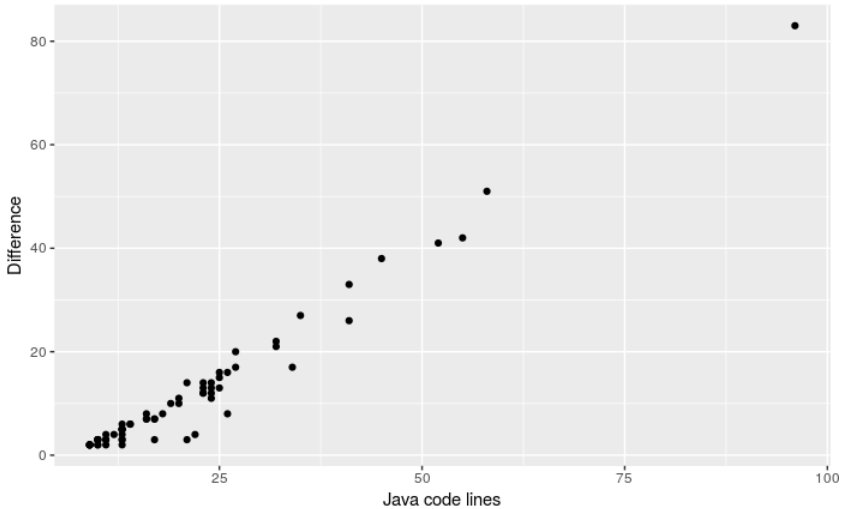
\includegraphics[width=.45\textwidth]
  {img/artigo_correlacao.jpg}
  \caption{\it Correlation between Java and Difference}
  \label{fig:correlacao}
\end{figure}

% Na Figure \ref{fig:geracao} é possível observar a geração de QDMs para 5 diferentes QCs. Para cada um deles foram gerados 6 QDMs, com diferentes quantidades de chamadores, 60, 100, 400, 700, 1000 e 2000.

In Figure \ref{fig:geracao} it is possible to observe the generation of QDMs for 5 different QCs. For each of them, 6 QMS were generated, with different amounts of callers, 60, 100, 400, 700, 1000 and 2000.

\begin{figure}[!ht] \centering
  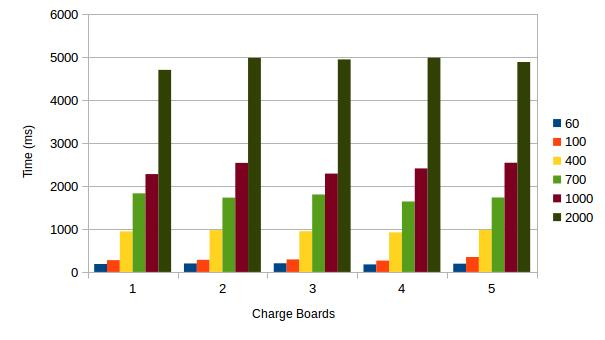
\includegraphics[width=.45\textwidth]
  {img/artigo_geracao.jpg}
  \caption{\it QDM Generation Time (ms)}
  \label{fig:geracao}
\end{figure}

\subsection{Results}

% Embora a RQ.3 não tenha sido respondida nesse trabalho, as outras duas foram respondidas de forma satisfatória. Ao analisar os dados relativos à RQ.1, foi possível observar que a representação de um chamador usando DSL é em média 45\% menor que a representação desse chamador em Java. Isso indica um possível ganho de produtividade para o testador, que terá que escrever uma quantidade menor de código. 

Although \textbf{RQ.3} was not answered in this study, the other two were satisfactorily answered. When analyzing the data related to RQ.1, it was possible to observe that the representation of a caller using DSL is on average 45\% smaller than the representation of this caller in Java. This indicates a possible productivity gain for the tester, which will have to write a smaller amount of code.

% A RQ.2 também foi respondida de forma satisfatória. O limite imposto pelo requisito funcional, de 5 segundos, não foi ultrapassado de forma expressiva nem quando foram usados 2000 chamadores, que é o dobro da quantidade de chamadores esperados para o sistema em produção.

\textbf{RQ.2} was also satisfactorily answered. The limit imposed by the functional requirement of 5 seconds was not exceeded expressively nor when 2000 callers were used, which is twice the number of callers expected for the system in production.

\subsection{Threats to validity}

% Foram usados apenas 66 chamadores reais, que serviram de base para medir o tempo de geração de QDMs. Espera-se que o SISDOT tenha por volta de 1000 chamadores, quando o mesmo estiver em ambiente de produção. Apesar da pequena quantidade de chamadores utilizada, incluindo suas repetições quando necessário, é esperado que o sistema cumpra o requisito funcional, pois os testes com o dobro de chamadores esperados ainda estão dentro do tempo máximo aceitável de 5 segundos para geração de QDM.

Only 66 real callers were used, which served as a basis for measuring the generation time of QDMs. SISDOT is expected to have around 1000 callers when it is in the production environment. Although the small number of callers used, including their repetitions when necessary, the system is expected to meet the functional requirement, since tests with twice as many expected callers are still within the maximum acceptable time of 5 seconds for QDM generation.

% A mesma situação ocorre com a comparação de linhas de código entre as declarações de chamadores em DSL e Java. Como a quantidade de chamadores é relativamente pequena, pode não ser possível generalizar os resultados encontrados.

The same situation occurs with the comparison of lines of code between the declarations of callers in DSL and Java. As the number of callers is relatively small, it may not be possible to generalize the results found.
